\section{Getting started}
\begin{frame}[fragile]
  \slidetitle

  In this section, we will learn how to:
  \begin{itemize}
    \item Configure git
    \item Clone a git repository
    \item Add a file to a repository
    \item Commit changes
    \item Undo modifications
    \item Undo staging
  \end{itemize}
    %A git repository contains a folder called {\bf .git}. There are two option to get a git repository:
%\begin{itemize}
%\item create a new repository using \cmd{git init}
%\item clone an existing git repository using \cmd{git clone}
%\end{itemize}
\end{frame}

\subsection{Configuring git}
\begin{frame}[fragile]
  \subslidetitle
  The global git configuration is stored in \cmd{~/.gitconfig}.
  \\
  \vspace{1em}

  The command \cmd{git config} can used to configure git:
  \begin{lstlisting}
$ (*\textcolor[HTML]{0000AA}{git config --global add user.name "My name"}*)
$ (*\textcolor[HTML]{0000AA}{git config --global add user.email "myemail@address"}*)
\end{lstlisting}

  Other git settings:
  \begin{lstlisting}[basicstyle=\small\ttfamily\bfseries]
$ (*\textcolor[HTML]{0000AA}{cat ~/.gitconfig}*)
[color]
  diff = auto
  status = auto
  branch = auto
  grep = auto

[alias]
  st = status
  co = checkout
  ci = commit
  br = branch
  l = log --graph --pretty=format:'%C(yellow)%h%C(cyan)%d%Creset %s %C(white)- %an, %ar%Creset'
  ll = log --stat --abbrev-commit

[merge]
  tool = kdiff3
  \end{lstlisting}
\end{frame}

%\subsection{git init}
%\begin{frame}[fragile]
  %\subslidetitle
  %The command \cmd{git init} is used to create a new repository.
  %The following steps create a new repository:
  %\begin{itemize}
  %\item run \cmd{git init} inside your project
    %\begin{itemize}
    %\item creates .git directory
    %\end{itemize}
  %\item Add files to git repository using \cmd{git add .}
  %\item Optional: add .gitignore file
  %\item Run {git commit} for initial commit
    %\begin{itemize}
    %\item creates branch called 'master'
    %\end{itemize}
  %\end{itemize}

%\begin{lstlisting}
%cd myproject
%git init
%git add .
%git commit
%\end{lstlisting}
%\end{frame}

\subsection{Obtaining a repository}
\begin{frame}[fragile]
  \subslidetitle
  The command \cmd{git clone} is used to download a whole git repository.
  \\
  \vspace{1em}
  Clone the gitmoon repository:
  \begin{lstlisting}
$ (*\textcolor[HTML]{0000AA}{git clone https://github.com/neolynx/gitmoon.git}*)
\end{lstlisting}

% protocols
%git protocols:
%\begin{itemize}
%\item http[s]
%\item ssh
%\item git
%\item ftp rsync ...
%\end{itemize}

  Let's see what we find in the working copy:
  \begin{lstlisting}
$ (*\textcolor[HTML]{0000AA}{cd gitmoon}*)
$ (*\textcolor[HTML]{0000AA}{ls}*)
moon_1024.jpg  moon.html  moon.js  three.min.js
\end{lstlisting}

  Oh, there is a HTML file !
  \begin{lstlisting}
$ (*\textcolor[HTML]{0000AA}{firefox moon.html \&}*)
\end{lstlisting}
\end{frame}

\subsection{Checking the status}
\begin{frame}[fragile]
  \subslidetitle

  The command \cmd{git status} shows the state of the local working copy:
  \begin{lstlisting}
$ (*\textcolor[HTML]{0000AA}{git status}*)
On branch master
Your branch is up-to-date with 'origin/master'.
nothing to commit, working directory clean
\end{lstlisting}
\end{frame}


\subsection{Adding a file}
\begin{frame}[fragile]
  \subslidetitle

  Let's create an AUTHORS file with your name:
  \begin{lstlisting}
$ (*\textcolor[HTML]{0000AA}{echo Tux Penguin > AUTHORS}*)
\end{lstlisting}

  Check the git status:
  \begin{lstlisting}
$ (*\textcolor[HTML]{0000AA}{git status}*)
On branch master
Your branch is up-to-date with 'origin/master'.
Untracked files:
  (use "git add <file>..." to include in what will be committed)

        (*\textcolor{red}{AUTHORS}*)

nothing added to commit but untracked files present (use "git add" to track)
\end{lstlisting}

\end{frame}
% --branch (different from master)
% --depth (shallow clone)
% --recursive (submodules)

\subsection{git add}
\begin{frame}[fragile]
  \subslidetitle

  The command \cmd{git add} tells git to track the file:
  \begin{lstlisting}
$ (*\textcolor[HTML]{0000AA}{git add AUTHORS}*)
\end{lstlisting}

  Check the git status:
  \begin{lstlisting}
$ (*\textcolor[HTML]{0000AA}{git status}*)
On branch master
Your branch is up-to-date with 'origin/master'.
Changes to be committed:
  (use "git reset HEAD <file>..." to unstage)

        (*\textcolor[HTML]{00AA00}{new file:}*)   (*\textcolor[HTML]{00AA00}{AUTHORS}*)
  \end{lstlisting}
\end{frame}


\subsection{git commit}
\begin{frame}[fragile]
  \subslidetitle

  The command \cmd{git commit} tells git to commit the file:
  \begin{lstlisting}
$ (*\textcolor[HTML]{0000AA}{git commit -m 'add authors file'}*)

[master c01af7f] add authors file
 1 file changed, 1 insertion(+)
 create mode 100644 AUTHORS
  \end{lstlisting}

  Check the git status:
  \begin{lstlisting}
$ (*\textcolor[HTML]{0000AA}{git status}*)
On branch master
Your branch is ahead of 'origin/master' by 1 commit.
  (use "git push" to publish your local commits)
nothing to commit, working directory clean
\end{lstlisting}
\end{frame}

\subsection{Git workflow}
\begin{frame}[fragile]
  \subslidetitle

  In this section, you

  \begin{itemize}
    \item cloned a repository
    \item added a file
    \item created your first commit
    \item leared the git commands: \cmd{clone}, \cmd{status}, \cmd{add} and \cmd{commit}
  \end{itemize}

  \centerline{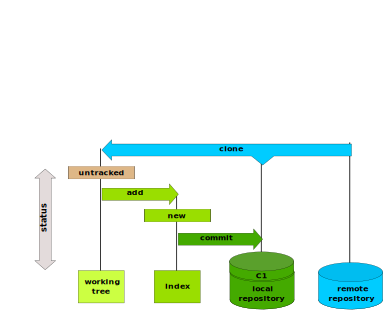
\includegraphics{diagrams/getting_started.pdf}}
\end{frame}


\subsection{Modifying a file}
\begin{frame}[fragile]
  \subslidetitle

  Let's change the \cmd{<title>} tag of \cmd{moon.html} to 'Git Moons':
  \begin{lstlisting}
$ (*\textcolor[HTML]{0000AA}{vi moon.html}*)
\end{lstlisting}

  Check the git status:
  \begin{lstlisting}
$ (*\textcolor[HTML]{0000AA}{git status}*)
On branch master
Your branch is up-to-date with 'origin/master'.
Changes not staged for commit:
  (use "git add <file>..." to update what will be committed)
  (use "git checkout -- <file>..." to discard changes in working directory)

        (*\textcolor{red}{modified:}*)   (*\textcolor{red}{moon.html}*)

no changes added to commit (use "git add" and/or "git commit -a")
\end{lstlisting}
\end{frame}

\subsection{git diff}
\begin{frame}[fragile]
  \subslidetitle

  The command \cmd{git diff} show the difference between working tree and index:
  \begin{lstlisting}
$ (*\textcolor[HTML]{0000AA}{git diff}*)
(*\textcolor[HTML]{00EE00}{diff --git a/moon.html b/moon.html}*)
(*\textcolor[HTML]{00EE00}{index d344c62..22e0c8e 100644}*)
(*\textcolor[HTML]{00EE00}{--- a/moon.html}*)
(*\textcolor[HTML]{00EE00}{+++ b/moon.html}*)
(*\textcolor[HTML]{0000EE}{@@ -1,7 +1,7 @@}*)
 <!DOCTYPE html>
 <html>
     <head>
(*\textcolor[HTML]{AA0000}{-}*)        (*\textcolor[HTML]{AA0000}{<title>moon</title>}*)
(*\textcolor[HTML]{00AA00}{+}*)        (*\textcolor[HTML]{00AA00}{<title>Git Moons</title>}*)
         <meta charset="utf-8">
  \end{lstlisting}
\end{frame}

\subsection{git add}
\begin{frame}[fragile]
  \subslidetitle

  The command \cmd{git add} tells git to stage the modifications:
  \begin{lstlisting}
$ (*\textcolor[HTML]{0000AA}{git add moon.html}*)
\end{lstlisting}

  Check the git status:
  \begin{lstlisting}
$ (*\textcolor[HTML]{0000AA}{git status}*)
On branch master
Your branch is up-to-date with 'origin/master'.
Changes to be committed:
  (use "git reset HEAD <file>..." to unstage)

        (*\textcolor[HTML]{00AA00}{modified:}*)   (*\textcolor[HTML]{00AA00}{moon.html}*)
  \end{lstlisting}
\end{frame}

\subsection{git commit}
\begin{frame}[fragile]
  \subslidetitle

  The command \cmd{git commit} tells git to commit the index to the local repository:
  \begin{lstlisting}
$ (*\textcolor[HTML]{0000AA}{git commit -m 'change title'}*)
[master fc92204] change title
 1 file changed, 1 insertion(+), 1 deletion(-)
\end{lstlisting}

  \centerline{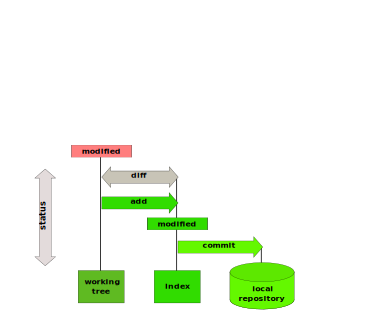
\includegraphics{diagrams/diff-modified-add-commit.pdf}}
\end{frame}

\subsection{Undo a modification}
\begin{frame}[fragile]
\subslidetitle

  Let's modify a file and verify the git status:
  \begin{lstlisting}
$ (*\textcolor[HTML]{0000AA}{echo "Tux le Pinguin" >> AUTHORS}*)
$ (*\textcolor[HTML]{0000AA}{git status}*)
On branch master
Your branch is up-to-date with 'origin/master'.
Changes not staged for commit:
  (use "git add <file>..." to update what will be committed)
  (use "git checkout -- <file>..." to discard changes in working directory)

        (*\textcolor{red}{modified:}*)   (*\textcolor{red}{AUTHORS}*)

\end{lstlisting}

  The command \cmd{git checkout} allows you to undo the modification:
  \begin{lstlisting}
$ (*\textcolor[HTML]{0000AA}{git checkout AUTHORS}*)
$ (*\textcolor[HTML]{0000AA}{git status}*)
On branch master
Your branch is up-to-date with 'origin/master'.
nothing to commit, working directory clean
\end{lstlisting}

Note: checkout discards the changes, handle with care!

\end{frame}

\subsection{Undo a modifaction}
\begin{frame}[fragile]
\subslidetitle
  \centerline{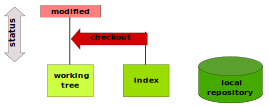
\includegraphics{diagrams/undo-modified}}
\end{frame}

\subsection{Undo staging}
\begin{frame}[fragile]
\subslidetitle

  Let's modify a file and stage it:

\begin{lstlisting}
$ (*\textcolor[HTML]{0000AA}{echo "Tux le Pinguin" >> AUTHORS}*)
$ (*\textcolor[HTML]{0000AA}{git add AUTHORS}*)
$ (*\textcolor[HTML]{0000AA}{git status}*)
On branch master
Your branch is up-to-date with 'origin/master'.
Changes to be committed:
  (use "git reset HEAD <file>..." to unstage)

        (*\textcolor[HTML]{00AA00}{modified:}*)   (*\textcolor[HTML]{00AA00}{AUTHORS}*)
\end{lstlisting}

The command \cmd{git reset} allows you to unstage a file:

\begin{lstlisting}
$ (*\textcolor[HTML]{0000AA}{git reset HEAD AUTHORS}*)
Unstaged changes after reset:
M       AUTHORS
\end{lstlisting}

\end{frame}

\subsection{git reset}
\begin{frame}[fragile]
\subslidetitle
  After \cmd{git reset}, the modification is still there:
\begin{lstlisting}
$ (*\textcolor[HTML]{0000AA}{git status}*)
On branch master
Your branch is up-to-date with 'origin/master'.
Changes not staged for commit:
  (use "git add <file>..." to update what will be committed)
  (use "git checkout -- <file>..." to discard changes in working directory)

        (*\textcolor{red}{modified:}*)   (*\textcolor{red}{AUTHORS}*)

no changes added to commit (use "git add" and/or "git commit -a")
\end{lstlisting}

  Instead of using \cmd{git checkout} on each file, the command \cmd{git reset --hard} to undo all modifications:
\begin{lstlisting}
$ (*\textcolor[HTML]{0000AA}{git reset --hard}*)
HEAD is now at fc92204 change title
\end{lstlisting}
\end{frame}

\subsection{Removing a file}
\begin{frame}[fragile]
\subslidetitle
  Let's first add a file:
\begin{lstlisting}
$ (*\textcolor[HTML]{0000AA}{touch test.file}*)
$ (*\textcolor[HTML]{0000AA}{git add test.file}*)
$ (*\textcolor[HTML]{0000AA}{git commit -m 'adding a test file'}*)
[master 3d0539f] add test file
 1 file changed, 0 insertions(+), 0 deletions(-)
 create mode 100644 test.file
\end{lstlisting}

  The command \cmd{git rm} removes a file from the repository:
\begin{lstlisting}
$ (*\textcolor[HTML]{0000AA}{git rm test.file}*)
rm 'test.file'
$ (*\textcolor[HTML]{0000AA}{git status}*)
On branch master
Your branch is ahead of 'origin/master' by 1 commit.
  (use "git push" to publish your local commits)
Changes to be committed:
  (use "git reset HEAD <file>..." to unstage)

        (*\textcolor[HTML]{00AA00}{deleted:}*)    (*\textcolor[HTML]{00AA00}{test.file}*)
\end{lstlisting}
\end{frame}

\subsection{git rm}
\begin{frame}[fragile]
\subslidetitle
  Commit the staged removal of the file:
  \begin{lstlisting}
$ (*\textcolor[HTML]{0000AA}{git commit -m 'we do not need the test file anymore'}*)
[master 06cb00f] remove test file
 1 file changed, 0 insertions(+), 0 deletions(-)
 delete mode 100644 test.file
\end{lstlisting}

\end{frame}

\subsection{Exercises}
\begin{frame}[fragile]
\subslidetitle
  Create a commit for each exercise below:
  \begin{exercise}
    \item Change the color of the moon to blue
    \item Change the \cmd{<h1>} tag of \cmd{moon.html} to 'Git Moons'
    \item Add a green moon

  \end{exercise}

\end{frame}

